% !TEX encoding = UTF-8
% !TEX TS-program = pdflatex
% !TEX root = ../tesi.tex

%**************************************************************
\chapter{Descrizione dello stage}
\label{cap:descrizione-stage}
%**************************************************************

\intro{Breve introduzione al capitolo}\\

%**************************************************************
\section{Introduzione al progetto}
\subsection{Descrizione del prodotto}
Il progetto ha come scopo la creazione di un’estensione del servizio MonoKee basato su \gls{blockchaing}. L’estensione offre un sistema di Identity Access Management (IAM) composto da quattro principali fattori:
    \begin{itemize}
        \item \textbf{Identity Wallet} (IW);
        \item \textbf{Service Provider} (SP);
        \item \textbf{Identity Trust Fabric} (ITF);
        \item \textbf{Trusted Third Party} (TTP);
    \end{itemize} 
In sintesi l’estensione dovrà operare al fine di fornire la possibilità ad un utente di registrare e gestire la propria identità autonomamente tramite l’IW e mandare i propri dati (PII) all’ITF, il quale custodirà la sua identità e farà da garante per le asserzioni provenienti dai TTP. Inoltre il SP dovrà essere in grado con le informazioni provenienti da IW e ITF di verificare o meno l’accesso ai propri servizi.
L'immagine in figura \ref{fig:diag-mod} dovrebbe chiarificare i vari componenti in gioco.
\begin{figure}[!h]
    \centering
    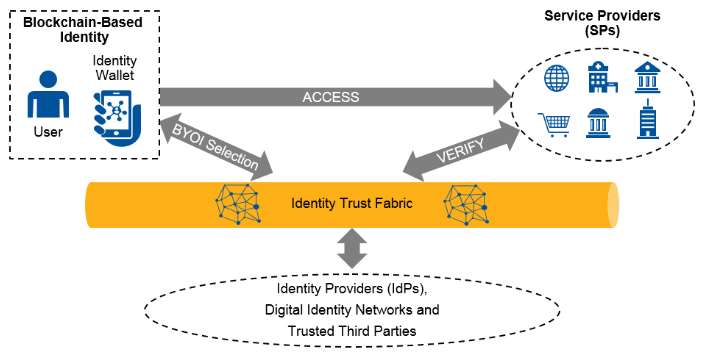
\includegraphics[width=0.9\columnwidth]{diagrammaComponenti.png} 
    \caption{Diagramma Moduli}
    \label{fig:diag-mod} 
\end{figure}
%**************************************************************
\section{Studio Tecnologico Identity Trust Fabric}

\subsection{Sintesi dello studio tecnologico}
Il capitolo procede descrivendo le caratteristiche del prodotto MonoKee e di come la tecnologia \gls{blockchaing} si possa collocare in tale contesto; vengono poi trattati i principali strumenti e librerie disponibili per sviluppare in Ethereum. L’analisi si conclude facendo emergere come un utilizzo di Ethereum sia possibile, ma non consigliato; le ragioni sono prettamente legate alla scalabilità del sistema. Per ragioni di facilità di sviluppo e di time to market si è ritenuto ad ogni modo di adottare la scelta di Ethereum come base del componente ITF.

\subsection{ITF – Identity Trust Fabric}
Sulla base di un primo studio di fattibilità l’unico componente coinvolto nell’uso \gls{blockchaing} è l’Identity Trust Fabric. La sua principale funzione è quella di poter permettere ai vari Service Provider aderenti al servizio di poter verificare le informazioni rilasciate dai vari utenti tramite l’utilizzo del loro personale Identity Wallet (IW). Il componente mantiene al suo interno l’hash della chiave pubblica degli utenti (che rappresenta la loro identità) e le asserzioni fornite dai vari IW che possono essere potenzialmente certificate da una TTP (tramite una firma con la loro chiave privata). Le asserzioni devono poter essere modificate o eliminate in ogni momento, naturalmente ogni alterazione deve essere di volta in volta certificata nuovamente. Anche da parte del TTP ci dev’essere la possibilità di revocare la certificazione di un’asserzione. 
Secondo lo studio Gartner in nota \footcite{farah:The-Dawn-of-Decentralized-Identity} una buona implementazione di una ITF deve possedere le seguenti caratteristiche:
\begin{itemize}
    \item \textbf{Fiducia}: il contenuto presente nella ITF deve essere solo quello autorizzato e non ci devono poter essere manomissioni malevoli da parte degli utilizzatori della rete. Ogni componente deve potere aver fiducia nella veridicità dei dati.
    \item \textbf{Garanzia}: le regole logiche della ITF non devono poter essere manomesse. Deve essere possibile applicare le varie policy aziendali in ambito di gestione dei rischi.
    \item \textbf{Tracciabilità}: ogni informazione e cambio di stato relativo alle identità e alle asserzioni deve poter essere tracciato e verificabile sia in termini cronologici sia in termini di provenienza. 
    \item \textbf{Sicurezza}: intesa come CIA. L’ITF deve rispettare i vincoli di confidenzialità, inalterabilità e disponibilità delle informazioni dentro lei contenute.
    \item \textbf{Scalabilità}: l’ITF deve fornire un elevato grado di scalabilità soprattutto in un’ottica in cui il prodotto potrebbe essere reso disponibile ad un uso Consumer.
    \item \textbf{Efficienza}: il funzionamento dell’ITF deve richiedere la minima quantità di risorse possibili.
\end{itemize}

\subsection{Introduzione alla tecnologia \gls{blockchaing}}
Al fine di rendere più consapevoli ai lettori le seguenti trattazioni si procede ad una esposizione ad alto livello dei principali concetti inerenti alla blockchain.
\emph{Blockchain} è comunenente definita come una base di dati distribuita composta da una serie di blocchi i quali possono contenere insiemi di dati o codice. In entrambi i casi questi sono temporalmente firmati.
Ogni blocco contiene l'hash del blocco precedente. In questo modo si crea una sorta di collegamento fra i blocchi che forma una catena, la cosidetta \emph{blockchain}. In questa catena solo il blocco successore può collegarsi al predecessore

Consideriamo, quindi, \emph{blockchain} una qualsiasi piattaforma informatica \textbf{distribuita} che possiede almeno le seguenti tre caratteristiche tecniche al fine di fornire un registro a prova di manomissioni: 
\begin{itemize}
    \item uso di funzioni crittografiche di \gls{hashg};
    \item uso di strutture dati con \emph{hash pointer};
    \item uso di protocolli di consenso distribuito.
\end{itemize}

L'uso di funzioni di hash e di strutture dati basate su \emph{hash pointers} conferisco a questa particolare tecnologia le sue peculiari caratteristiche di immutabilità dei dati e di conseguenza la rendono abile a fornire un registro a prova di manomissioni. Un registro con queste caratteristiche costituisce a sua volta un'affidabile struttura dati in grado di immaganizzare qualsiasi tipo di dato. Questo rende anche possibile l'aggiungere di nuovi dati in coda al registro. 

Chiunque tenti di modificare un qualsiasi punto della blockchain, renderà in questo modo l'\emph{hash pointers} presente nel nodo successore errato. Se costudiamo la testa della catena, anche se l'attacante modifica i nodi successivi della catena in modo da renderli consistenti all'alterazione che ha cercato di intrurre, saremmo comunque in grado di identificare la manomissione verificando la corretezza del puntatore di testa.

Altra caratteristica fondamentale è l'uso di un alogoritmo di consenso distribuito, questo rende possibile lo sviluppo di applicazioni distribuite; le cosidette \emph{dapp}. Una \emph{dapp} imaggazzina i propri dati e i propri registri delle operazioni in una \emph{blockchain} in modo di evitare qualsiasi qualsiasi punto di vulnerabiltà singolo (\emph{single point of failure}). Un ottimo esempio di \emph{dapp} può essere una qualsiasi cripto-moneta.

\subsubsection{Funzione crittografica di hash}
Una funzione di hash è una funzione matematica che converte un input di qualsiasi lunghezza in un output di lunghezza definita efficacemente. Una funzione di hash per essere considerata sicura deve possedere almeno le seguenti caratteristiche:
\begin{itemize}
    \item essere invertibile;
    \item resistente alle collisioni;
    \item essere puzzle-friendly.
\end{itemize}
Essere invertibile significa che non ci dev'essere nessun algoritmo tecnicamente fattibile in grado di identificare l'input dall'output.
Essere resistente alle collisioni significa che non ci dev'essere nessuna tecnica in grado di individuare casi in cui a due input differenti corrispenda uno stesso output. Questo non inplica che la funzione debba essere iniettiva.
Essere puzzle-friendly significa che la tecniche più facile per inveritire una funzione di hash è quella del \emph{brute forcing}. Questa ultima caratteristicha risulta fondamentale nel contesto dell'algoritmo di consenso.

\subsubsection{Puzzle di ricerca}
Il puzzle di ricerca consiste in un problema matematico che per essere risolto necessità di una ricerca della soluzione in un vasto dominio. Si dice che un puzzle di ricerca è puzzle-friendly quando non è presente nessuna strategia migliore rispetto al provare valori casuali. Questo tipo di problemi computazionali vengono adottati da alcune \emph{blockchain} come base delle cosidette \gls{powg}, particolari algoritmi di consenso nei quali i vari nodi della rete competono per la risoluzione del problema. L'attuazione di questo algoritmo rende possibile la decentralizzazione. Nelle \emph{blockchain} basate su \gls{powg} il nodo che riesce a risolvere il puzzle per primo viene riconosciuto come prossimo nodo che inserirà un blocco nella catena 

\subsubsection{Commitment}
Un \emph{commitment} è l'equivalente digitale di leggere un valore, sigillarlo in una busta e poi metterla in un luogo sicuro. Il valore prelevato rimane segreto agli altri nodi fino a che il nodo che ha effettuato il \emph{commitement} non decida di rivelarlo. Le due funzioni che rendona questo possibile sono il \textbf{commit} e la \textbf{verify}.

Il \emph{commit} è una funzione che prende un messaggio e un numero randomico secrete ( \gls{nonceg}\glsfirstoccur) come input e ritorna un  \emph{commitment}.

La \emph{verify} è una funzione che prende \emph{commitment}, \gls{nonceg} e messaggio come input. Restituisce \emph{true} in caso la funzione di \emph{commit} con input il messaggio e il nonce passati abbia un output corrispondente al commitment fornito. In tutti gli altri casi ritorna \emph{false}.

Per usare questo schema abbiamo come primo passo quello di generare un numero randomico in qualità di nonce. Poi ci usando la funzione \emph{commit} pubblichiamo un \emph{commitment} usando il nonce appena generato. In un secondo momento, quando vogliamo rivelare il valore commitato in precedenza, pubblicheremo il nonce e il messaggio usati con la funzione di \emph{commit}. Una terza parte potrà poi essere in grado di verificare il messaggio tramite l'uso della funzione \emph{verify}.
Questa particolare tecnica risulta particolarmente utile al fine di immaganizzare le identità o attributi su di essa all'interno della \emph{blockchain}. Un \emph{commitment} per essere tale deve nascondere le informazioni. Questa significa che non potranno più essere alterate. 

\subsubsection{Strutture dati con hash pointer}
Un \emph{hash pointer} è un puntatore verso il posto dove un dato è contenuto, unito al valore del dato sotto forma di hash. A differenza di un normale puntatore che è solo in grado di fornirti un modo per ottenere l'informazione, un \emph{hash pointer} permette anche di essere in grado di capire se il particolare dato è stato alterato dalla creazione del puntatore. Questo particolare puntato può essere usato per la creazione di tipiche strutture dati concatenate, quali liste e alberi. La \emph{blockchain} è una lista concatenata(\emph{linked list}) costruita usando \emph{hash pointer} in vece ai classici puntatori. In una \emph{blockchain}, ogni blocco non solo ci dice dove si trova il blocco precedente, ma ci fornisce anche il valore dell'hash di questo blocco permettendoci quindi di poter verificare qualsiasi alterazione. Le particolari caratteristiche degli \emph{hasp pointer} usati ci permette di verificare l'intera catena a partire dal blocco di testa del quale ci dobbiamo fidare. 
Un'immagine esplicativa di quanto appena detto è presente in figura \ref{fig:linked-list}

\begin{figure}[!h]
    \centering
    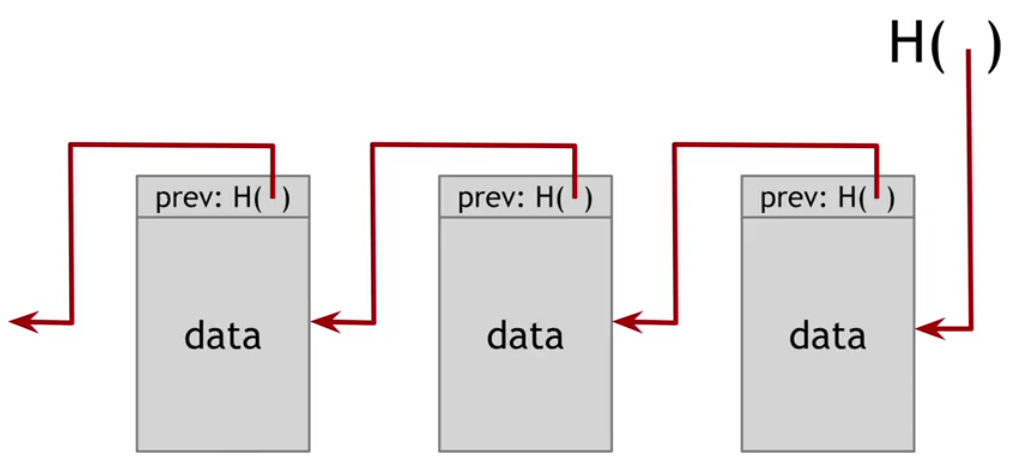
\includegraphics[width=0.9\columnwidth]{linked-list.png}
    \caption{Lista concatenato con \emph{hash pointer}}
    \label{fig:linked-list} 
\end{figure}

\subsubsection{Albero di Merkle}
Comunamente le principali \emph{blockchain} fanno uso di una particolare struttura dati per immagazzinare la loro componente di dati, l'albero di Merkle. L'albero di Merkle è un albero binario che usa \emph{hash pointer} in sostituzione dei classici puntatori. I record in quest'albero sono strutturati in coppie, e i loro hash conservati un livello superiore. Questa definizione si applica ad ogni livello del nodo fino al raggiungimento della radice. Le foglie rappresentano i dati. La figura \ref{fig:markle-tree} dovrebbe esporre con chiarezza il concetto.

\begin{figure}[!h]
    \centering
    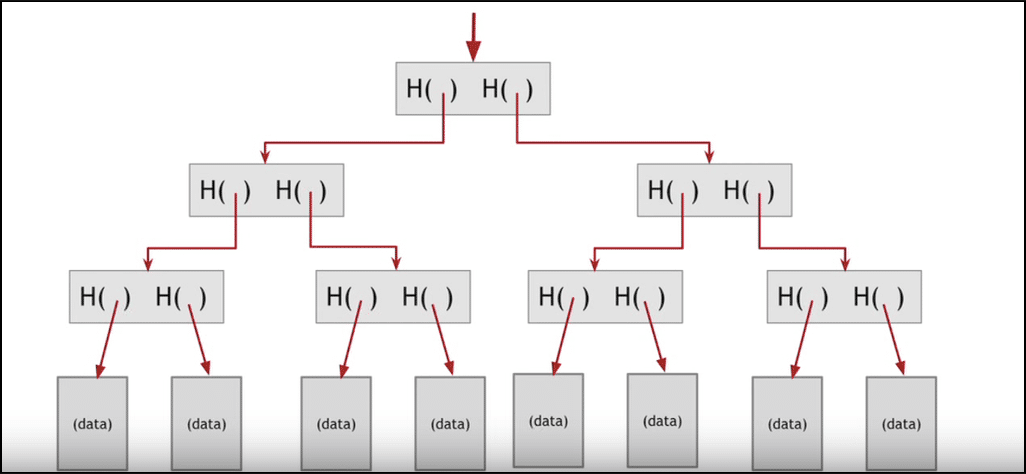
\includegraphics[width=0.9\columnwidth]{merkle-tree.png}
    \caption{Albero di Merkle}
    \label{fig:merkle-tree} 
\end{figure}

In caso di alterazioni in un qualsiasi nodo dell'albero queste sarebbero rilevabile in quanto causerebbero delle incoerenze nei puntatori presenti nei nodi al livello superiore. L'uso di questa struttura nel contesto di una \emph{blockchain} semplifica la verifica dell'attribuzione dei blocchi e permette di dover conservare solo la radice nel blocco di testa.

\subsubsection{Algoritmo di consenso}
\label{cap:alg-cons}
Abbiamo visto come l'uso di funzioni di hash e di strutture dati particolari rendono la \emph{blockchain} un'affidabile e verificabile base di dati centralizzata. Uno dei principali fattori di successo della tecnologia è stata però la natura decentralizzata di essa. Questa è possibile grazie all'uso di molteplici nodi in sostituzione ad un server centralizzato. La presenza di un algoritmo di consenso rende possibile ai vari nodi partecipanti accordarsi su cosa debba essere scritto o meno nella catena. Assumento che i vari nodi (anche malevoli) ricevano un input valido l'algoritmo di consenso assicura le seguenti proprietà:
\begin{itemize}
    \item l'algoritmo termina quando tutti i nodi onesti sono in accordo sul valore;
    \item l'algoritmo assicura che il valore è stato prodotto da un nodo onesto. 
\end{itemize}

In questo caso, un nodo onesto viene scelto per inserire il proprio blocco in cosa alla catena. In questo modo, l'algoritmo permette al sistema di generare fiducia in un contesto in cui nessun nodo si fida dell'altro.

Tipicamente in una \emph{blockchain} avvengono le seguenti operazioni. A intervalli regolari, ogni nodo propone le proprie transazioni in sospeso per essere inserite come prossimo blocco. Successivamente si attua l'algoritmo di consenso in cui ogni nodo proprone come input il blocco che intendono inserire. Alcuni nodi potrebbero essere malevoli e inserire transazioni non valide nei proprio blocco di input, ma possiamo assumere che gli altri nodi sono onesto. Se l'algoritmo di consenso ha successo viene selezionato il blocco da inserire in coda. Nessuno decide quale sarà il prossimo nodo ad essere inserito nella blockchain.

C'è comunque da ricordare che la presente è una trattazione ad alto livello, e quindi non verranno presentati particolari algoritmi di consenso. Mi limito quindi a presentare le principali carattestiche che questo deve avere:
\begin{itemize}
    \item equità;
    \item velocità;
    \item dimostrabilità;
    \item resistenze al problema dei generali bizantini;
    \item efficente;
    \item resistente ad attacchi Dos e DDos.
\end{itemize}

\subsection{Permissionless e Permissioned \gls{blockchaing}}
Al fine di poter valutare la fattibilità dell’utilizzo di Ethereum quale \gls{blockchaing} sottostante all’ITF è necessario avere in mente le due principali categorie di \gls{blockchaing}: \textbf{permissionless} e \textbf{permissioned}.

\subsubsection{Permissioned \gls{blockchaing}}
Una permissioned \gls{blockchaing} pone dei vincoli sulla partecipazione alla rete. Solo i nodi autorizzati possono partecipare all’algoritmo di consenso dei blocchi. Le autorizzazioni possono essere date singolarmente quindi i vari nodi possono avere o meno le seguenti possibilità:
\begin{itemize}
    \item lettura dei blocchi;
    \item scrittura dei blocchi;
    \item esecuzione di codice (se prevista dalla \gls{blockchaing});
    \item verifica dei nodi.
\end{itemize}

\subsubsection{Permissionless blockchaing}
Una permissionless \gls{blockchaing} è una rete in cui qualsiasi nodo può partecipare al processo di verifica dei blocchi. Ogni nodo ha tutte le precedenti quattro proprietà.

\paragraph{Ethereum}
Ethereum è una piattaforma decentralizzata pubblica ed open-source basata sulla creazione di \gls{SmartContractg}. Permette la creazione di applicazioni che operano su \gls{blockchaing} in modo che non ci sia alcuna possibilità di downtime, censura, frodi o interferenze da terze parti. Rappresenta una dei principali esempi di rete permissionless.
La piattaforma è stata rilasciata nel corso del 2014 ed è mantenuta dalla Ethereum Foundation, e questo fa di Ethereum una delle più longeve \gls{blockchaing} disponibili. Ciò comporta la presenza di una documentazione abbastanza nutrita rispetto ai competitor e di un buon numero di strumenti già disponibili. 
L’elevata popolarità della tecnologia e alcune sue caratteristiche non presenti nei competitor, ha fatto sì che una notevole quantità di sviluppatori abbiano deciso di utilizzarla. Il sito \footnote{site:state-dapps} mantiene una vetrina di oltre milleseicento esempi. Sono presenti tutte le più significative applicazioni ora in produzione; si fa notare che molte di esse sono state le fonti dei più diffusi pattern Ethereum.

\paragraph{Programmare SmartContract}
Solidity è il principale linguaggio di programmazione usato per scrivere \gls{SmartContractg}. Nonostante sia presente un’implementazione basata su Go, questa è ancora acerba e non largamente utilizzata e per questo motivo tale implementazione non verrà trattata nel documento.
Solidity è un linguaggio di programmazione ad oggetti ad alto livello. Il suo sviluppo è stato fortemente influenzato da linguaggi quali C++, Python e Javascript. Gli SmartContract così scritti vengono poi trasformati in bytecode e quest’ultimo viene eseguito dall’Ethereum Virtual Machina (EVM).
Il linguaggio seppur non completamente maturo offre la maggior parte delle caratteristiche tipiche di un linguaggio ad oggetti. Infatti Solidity è fortemente tipato, supporta l’ereditarietà, librerie esterne e tipi definiti dall’utente. A sottolineare la bontà del linguaggio si evidenzia come in Solidity sia presente il concetto di interfaccia, caratteristica non presente in linguaggi ben più longevi. 
Queste caratteristiche rappresentano un notevole vantaggio per Ethereum rispetto ai diretti competitor, i quali spesso utilizzano linguaggi acerbi e/o a basso livello. Si è ritenuto che un linguaggio con le caratteristiche precedentemente descritte sia fondamentale per la buona riuscita del progetto, soprattutto in un’ottica di manutenibilità e estendibilità.
\paragraph{Breve nota sull'applicabilità dei pattern}
Nonostante il linguaggio permetta l’applicabilità dei più diffusi pattern si vuole far notare come nel contesto di una blockchain Permissionless questi risultino spesso controproducenti. 
Durante la progettazione e l’applicazione dei pattern vanno sempre ricordati i seguenti punti:
\begin{itemize}
    \item l’esecuzione di un metodo che modifica la blockchain si paga in base al lavoro che viene effettivamente svolto;
    \item complessità lineari portano a costi difficilmente accettabili;
    \item plugin come Metamask calcolano il massimo costo possibile di una transazione, in caso il credito non sia sufficiente la transazione fallisce. Ne condegue che un ciclo for su una lista di un elemento viene stimato presupponendo che la lista sia completamente piena;
    \item la velocità di esecuzione varia in base alla somma pagata per questa, anche con somme estremamente alte o su reti locali i tempi potrebbero essere considerati non giustificabili per la maggior parte degli utenti;
    \item ogni oggetto e campo dato si paga in base al loro spazio occupato;
    \item il costo della moneta e quindi delle transazioni è fortemente variabile. Approcci che, oggi risultano economici, possono diventare economicamente insostenibili a distanza di pochi giorni.
\end{itemize}
A seguito dei precedenti punti dovrebbe risultare più evidente come pattern che prevedono alta complessità temporale e spaziale siano inaccettabili su una rete Ethereum. Ad esempio i pattern Command e Decorator risultano difficilmente giustificabili.
Sono invece presenti pattern pensati appositamente per Ethereum, questi sono presenti nella documentazione ufficiale Solidity \footcite{site:solidity-documentation}. Particolarmente utili al contesto del progetto in esame ritengo possano essere utili i seguenti pattern: 
\begin{itemize}
    \item Owner Pattern;
    \item Vote Pattern 
    \item WhiteList Pattern.
\end{itemize}

\paragraph{Complessità e pratiche non convenzionali}
\label{cap:prestazioni}
I punti precedentemente stilati nel paragrafo sull’applicabilità dei pattern portano anche delle notevoli differenze in termini di pratiche di stile di programmazione. Tra queste riporto:
\begin{itemize}
    \item l’uso di liste e array è fortemente sconsigliato, vanno preferite strutture dati con accesso costante. Solidity fornisce il tipo mapping;
    \item la creazione di oggetti (in termini Solidity contratti) ha un costo notevole. Una buona pratica è quella di utilizzare ADT (Abstract Data Type) differenti, come le strutture;
    \item cicli for che portano complessità lineare dovrebbero essere evitati, elaborazioni di questo tipo dovrebbero essere affidate a server esterni o a livello client-side;
    \item l’utilizzo dei puntatori (in Solidity address) nasconde completamente il tipo dell’oggetto puntato rendendo vano il controllo dei tipi. Andrebbe evitato il più possibile.
\end{itemize}
Si fa notare come in particolare l’ultimo punto degeneri completamente il concetto di programmazione ad alto livello.

\paragraph{Strumenti}
Vista la relativa maturità della tecnologia, esistono diversi strumenti utili:
\begin{itemize}
    \item \textbf{Truffle}: è una suite di development e testing. Permette di compilare, buildare ed effettuare la migrazione degli SmartContract. Inoltre ha funzioni di debugging e di scripting. La suite offre la possibilità di effettuare test degli SmartContract sia in Javascript (con l’utilizzo di Chai), sia in Solidity. Si riporta di seguito il sito del progetto: \cite{site:truffle}.
    \item \textbf{Ganache}: è uno strumento rapido che permette di creare e mantenere in locale una rete blockchain Ethereum personale. Può essere usata per eseguire test, eseguire comandi e per operazioni di controllo dello stato mentre il codice esegue. Si riporta di seguito il sito del progetto: \cite{site:ganache}.
    \item \textbf{Mist}: è un browser sviluppato direttamente dal team Ethereum in grado di operare transazioni direttamente nella blockchain senza la necessità di possedere un intero nodo. È estremamente immaturo e non utilizzabile in produzione. Si riporta di seguito il sito del progetto: \cite{site:mist}.
    \item \textbf{Parity}: è un client Ethereum che permette di operare sulla rete senza necessità di possedere un intero nodo. Questa soluzione a differenza di Mist dovrebbe risultare più facilmente integrabile nel prodotto senza che l’utente ne abbi consapevolezza. Si riporta di seguito il sito del progetto: \cite{site:parity} .
    \item \textbf{Metamask}: è uno plugin disponibile per i browser Chrome, Firefox, e Opera. Permette di interfacciarsi alla rete Ethereum senza la necessità di eseguire in intero nodo della rete. Il plugin include un wallet con cui l’utente può inserire il proprio account tramite la chiave privata. Una volta inserito l’account il plugin farà da tramite tra l’applicazione e la rete.
    Metamask è utilizzato dalla maggioranza delle applicazioni Ethereum presenti on line, questo però rappresenterebbe un componente esterno compatibile con pochi browser desktop. Si riporta di seguito il sito del progetto: \cite{site:metamask} .
    \item \textbf{Status}: è un progetto che propone una serie di \gls{apig} che permettono di sviluppare un’applicazione mobile nativa operante direttamente su blockchain senza la necessità di possedere un intero nodo. Il sito del progetto propone una serie di applicazioni che utilizzano Status. Tuttavia nessuna di queste applicazioni risulta attualmente rilasciate in nessuno store. Status risulta in early access ed è disponibile per Android e iOS. Il sito del progetto è il seguente: \cite{site:status}.
    \item \textbf{Microsoft Azure}: “Ethereum Blockchain as a Service” è un servizio fornito da Microsoft e ConsenSys che permette di sviluppare a basso costo in un ambiente di dev/test/produzione. Permette di creare reti private, pubbliche e di consorzio. Queste reti saranno poi accessibili attraverso la rete privata Azure. Questa tecnologia rende facile l’integrazione con Cortana Analytics, Power BI, Azure Active Directory, O365 e CRMOL.
\end{itemize}

\paragraph{Valutazione applicabilità soluzione Ethereum}
Al fine di poter valutare correttamente da ogni punto di vista l’applicabilità di una soluzione basata su Ethereum quale base della componente ITF, si procede ad analizzare in maniera analitica le sei caratteristiche presentate nel capitolo ‘ITF – Identity Trust Fabric’.

\begin{itemize}
    \item \textbf{Fiducia} \\
    Questa caratteristica è ottenuta da Ethereum da una combinazione di diversi fattori quali:
    \begin{itemize}
        \item utilizzo di incentivi economici, il pagamento per effettuare operazioni;
        \item utilizzo di prove di interesse (Proof of Interest).
    \end{itemize}
    Le prove di interesse possono essere di due tipi:
    \begin{itemize}
        \item Proof of Stake, l’esibizione di un interesse;
        \item Proof of Work, l’uso di potenza di calcolo per risolvere un problema matematico.
        Queste metodologie fanno in modo che solo chi realmente interessato possa influenzare l’algoritmo di consenso dei blocchi. Questo rende minore la possibilità di un "51 percent attack" \footcite{site:51-attack}. C’è comunque da ricordare che un attacco di questo tipo e praticamente impossibile.
    \end{itemize}
    Per queste ragioni si ritiene una rete Ethereum sia completamente soddisfacente per quanto riguarda l’aspetto fiducia al pari di una rete di tipo permissioned.
    \item \textbf{Garanzia}\\
    Lo studio\footcite{farah:The-Dawn-of-Decentralized-Identity} evidenzia come questo rappresenti un punto critico. Infatti riporta che il raggiungimento di questo obiettivo è fortemente condizionato dall’efficacia dell’algoritmo di consenso e dai nodi presenti nella rete. Lo studio prosegue facendo notare che la presenza di nodi malevoli, oltre che mettere a rischio l’algoritmo di consenso, può compromettere anche il corretto funzionamento dell’ITF. Trattandosi infatti di una blockchain pubblica ogni nodo è in grado di visionare il contenuto di ogni singolo contratto, inclusi i dati e i metodi presenti. Per quanto riguarda i dati questo potrebbe non essere un problema in quanto si può immagazzinare una versione codificata del dato. Per quanto riguarda i metodi invece questo non è possibile, ed anzi, potrebbe rendere in grado ad un attaccante di trovare eventuali bachi e criticità dell’ITF. Il servizio Azure potrebbe permette di creare reti private.
    \item \textbf{Tracciabilità}\\
    Lo studio Gartner\footcite{farah:The-Dawn-of-Decentralized-Identity} evidenzia come in una rete permissionless la tracciabilità temporale non sia possibile, questo perchè in una rete distribuita ogni nodo può avere un concetto di tempo proprio. Questo però non risulta possibile in nessun approccia risolutivo all’ITF basato su blockchain, infatti le reti permissioned applicano timestamp a livello di blocco e non di transazione. Anche ammettendo che ci sia un concetto di tempo comune tra i nodi, le transizioni rimarrebbero temporalmente non tracciabili. La cosa potrebbe permettere ad un blocco di alterare l’ordine delle transazioni. 
    Tale complicazione in una rete permissioned può essere superata creando blocchi immutabili e ogni qual volta si voglia fare una modifica, si dovrà creare un nuovo blocco. In questo modo ci sarà solo una transazione di creazione blocco il cui timestamp coinciderà con il timestamp del blocco.
    L' approccio in Ethereum rimane in ogni caso impraticabile. Attualmente non sono note ulteriori tecniche per la tracciabilità temporale in Ethereum, motivo per cui l’attribuzione di un riferimento temporale dovrà essere effettuato lato client, con i conseguenti limiti di sicurezza. 
    \item \textbf{Sicurezza}\\
    La confidenzialità dei dati, anche se non presente nativamente in Ethereum, è facilmente ottenibile immagazzinando nei contratti solo un hash dei dati.
    L’integrità dei dati invece è garantita dalla prova di lavoro che utilizza la blockchain come già ribadito nella sezione Fiducia.
    La disponibilità invece è garantita dalle caratteristiche di distribuzione di ogni blockchain.
    Un ulteriore punto di considerazione da fare è che chiunque ha la possibilità di vedere il contenuto di ogni SmartContract incluso il codice dei metodi. Questo come già detto può comportare la possibilità da parte di un attaccante di individuare eventuali errori logici. Ogni contratto dovrà comunicare con gli altri attraverso chiamate a metodi pubblici, in quanto non c’è in Ethereum nessun concetto di visibilità dei metodi di tipo protected o package. Questo rende possibile da parte di qualsiasi utente della rete di utilizzare questi metodi in maniera malevole. Questo tipo di problematica è facilmente superabile applicando i dovuti pattern Solidity quali WhiteList Pattern e Owner Pattern. L’applicazione dei pattern però comporterebbe un notevole aumento in termini di complessità e costo soprattutto in presenza di logiche di accesso variegate e dinamiche. Inoltre, in caso di liste di utenti autorizzati, queste potrebbero risultare onerose in termini di costo.
    \item \textbf{Scalabilità}\\
    Ethereum per poter applicare l’algoritmo del consenso, fa utilizzo di una prova di lavoro che deve essere fatta in occasione di ogni transazione. La prova consiste nella risoluzione di un problema crittografico la cui difficoltà è dinamica in base a diversi fattori della blockchain, quali valore dell’Ether, numero di utenti, numero di transazioni, etc. Oltretutto si nota come anche in lettura ci sia una lentezza che difficilmente potrebbe essere ritenuta accettabile da un utente medio. Per avere prova di questo fatto si può prendere in esame una qualsiasi Dapp presente al seguente link \footcite{site:state-dapps}. La questione pone anche limiti, come già citato, in termini di costo.
\end{itemize}
\subsection{Conclusioni}
Da quanto è emerso l’utilizzo della tecnologia Ethereum quale base dell’ITF, pone una serie di vantaggi e svantaggi. Di seguito si propone una sintetica trattazione dei punti fondamentali, per maggiori dettagli si consiglia la lettura dell’intero documento.
I vantaggi sono:
\begin{itemize}
    \item Ethereum offre un linguaggio ad alto livello e ad oggetti a differenza di altri competitor;
    \item Ethereum offre una notevole maturità e anche un’ampia platea di strumenti, molti dei quali estremamente maturi e largamente utilizzati.
\end{itemize}
    
Gli svantaggi sono: 
\begin{itemize}
    \item Ethereum è una rete pubblica, non è possibile fare nessuna restrizione di privilegi sui nodi partecipanti alla rete. Ciò potrebbe rappresentare un problema di sicurezza;
    \item la comunicazione verso dispositivi mobili non è verificabile da quest’ultimi, in quanto dovrebbe avvenire tramite comunicazione REST;
    \item sono presenti forti limitazioni in termini di costo e velocità, il sistema risulterebbe lento ed estremamente costoso. Ciò comporta notevoli difficoltà sulla scalabilità del servizio.
\end{itemize}
Si ritiene che un approccio basato sul Ethereum sull’ITF sia possibile, le eventuali criticità di sicurezza e fiducia verso i dispositivi mobili sono superabili con una buona progettazione. L’unico fattore veramente critico rimane la scalabilità del sistema, fatto che, a mio parere, è sufficiente per ritenere Ethereum non adatto all’utilizzo, soprattutto in un’ottica commerciale. Quindi se pure possibile, non si consiglia l’utilizzo di Ethereum. Per ragioni di facilità di sviluppo e di time to market si è ritenuto comunque di adottare la scelta di Ethereum come base del componente ITF.

%**************************************************************

\section{Studio di fattibilità Identity Wallet}
\subsection{Sintesi dello studio di fattibilità}
Lo studio inizia descrivendo come l’IW si cali in questo contesto. Si prosegue prendendo in considerazione le alternative di sviluppo mobile e Desktop. A seguito di un’analisi dei possibili utenti emerge una netta preferenza per lo sviluppo mobile.
Vengono poi trattati i principali strumenti e librerie disponibili per lo sviluppo ed è consigliabile uno sviluppo multi piattaforma, con target Android e iOS. In conclusione emerge una preferenza per il framework Xamarin.
\subsection{Descrizione componente Identity Wallet} 
Il progetto ha come scopo la creazione di un Identity Wallet (IW). L’applicativo si colloca nel contesto di un’estensione del servizio Monokee basato su blockchain. L’estensione offre un sistema di \gls{iamg} composto da quattro principali fattori:
\begin{itemize}
    \item Identity Wallet (IW)
    \item Service Provider (SP)
    \item Identity Trust Fabric (ITF)
    \item Trusted Third Party (TTP)
\end{itemize}
    
In sintesi, l’estensione dovrà operare al fine di fornire la possibilità ad un utente di registrare e gestire la propria identità automatamente tramite l’IW, mandare i propri dati (IPP) all’ITF la quale custodirà la sua identità e farà da garante per le asserzioni proveniente dai TTP. Inoltre il SP dovrà essere in grado, con le informazioni provenienti da IW e ITF, di garantire o meno l’accesso ai propri servizi.
Il software IW, più dettagliatamente, dovrà assolvere i seguenti compiti:
nell’ambito della registrazione di un utente il Wallet deve:
\begin{itemize}
    \item generare e immaganizzare in locale una chiave pubblica;
    \item generare e immaganizzare in locale una chiave private;
    \item creare l’hash della chiave pubblica e inviarla all’ITF;
    \item incrementare le informazioni (PII) relative alle identità che il Wallet gestisce.
\end{itemize}
Nell’ambito della presentazione dei dati ad un Service Provider deve:
\begin{itemize}
    \item invio della chiave pubblica al service provider;
    \item invio di un puntatore all’hash della chiave pubblica interna al ITF;
    \item invio di altre informazioni utili presenti nel ITF;
    \item gestire ulteriori layer di sicurezza, quali impronta digitale, QR code, autentificazione multi fattore)
\end{itemize}
nell’ambito della richiesta di accesso ad un servizio deve:
\begin{itemize}
    \item inviare una richiesta di accesso ad un servizio con i dati relativi all’identità al Service Provider;
    \item attendere la risposta del Service Provider.
\end{itemize}

\subsection{Studio del dominio}
\subsubsection{Dominio Applicativo}
L’applicativo IW dovrà essere usato in un contesto prevalentemente lavorativo. Non si escludono però ulteriori applicazione future in ambito Consumer. In ogni caso è indirizzato a utenti senza specifiche conoscenze informatiche e con minimo training tecnologico. Il software quindi dovrà essere il più accessibile e semplice possibile e per tali ragioni si pensa ad un suo utilizzo prevalentemente in ambito mobile, anche se non si esclude a priori la possibilità di una versione Desktop. L’applicativo mobile deve essere disponibile per la più ampia gamma di utenti possibili.
\subsubsection{Dominio Tecnologico}
Un eventuale applicativo Desktop ha un’elevata probabilità di non rientrare nei tempi dello stage, motivo per la quale si è deciso di non tenerlo in considerazione. L’applicativo quindi dovrà essere fruibile tramite un’applicazione mobile multipiattaforma sviluppabile entro i limiti temporali della durata dello stage. 
Per queste ragioni lo studio del dominio tecnologico si incentrerà principalmente su tecnologie multi piattaforma mobili. Verrà comunque tenuto in considerazione anche lo sviluppo nativo.
\paragraph{Studio diffussione sistemi operativi mobili}
Procedo di seguito ad un’analisi sulla diffusione dei vari sistemi operativi mobili.
I dati in figura ~\ref{fig:diff-os-mob} riportati provengono da Kantar \footcite{site:kantar-study} società di analisi inglese e fanno riferimento al trimestre che va da novembre 2016 a gennaio 2017.
\begin{figure}[!h] 
    \centering
    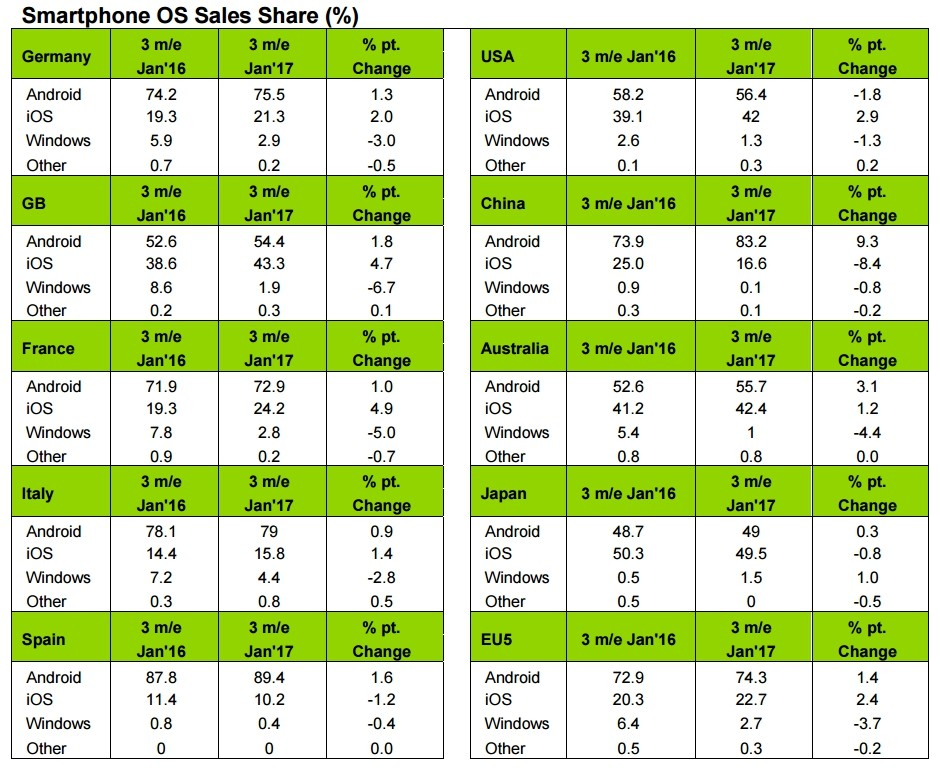
\includegraphics[width=0.9\columnwidth]{diff-os-mob.png} 
    \caption{Diffuzione sistemi mobili}
    \label{fig:diff-os-mob} 
\end{figure}
Da come si può evincere dai dati, Android, iOS, Windows Phone rappresentano, in questa sequenza ed in ogni mercato, i sistemi più diffusi. I restanti sistemi non raggiungono cifre significative. Ponendo maggiore attenzione ai primi tre sistemi si nota come Android nell’area EU5 rappresenti i tre quarti del mercato. In Giappone, Stati Uniti, Australia e Gran Bretagna invece la situazione risulta più bilanciata con una sostanziale parità. Windows Phone in ogni mercato si pone in terza posizione con percentuali che non superano mai l’otto percento. Individuando nell’area EU5 il principale mercato per MonoKee si ritiene che il prodotto IW debba essere sviluppato per i sistemi Android e iOS, dando la precedenza al primo. Non si ritiene necessario lo sviluppo di un’applicazione Windows Phone in quanto difficilmente attuabile nei tempi dello stage. 
\paragraph{Tecnologie per lo sviluppo}
Segue un approfondimento relativo alle potenziali tecnologie con cui sviluppare l’IW. Data la necessità di sviluppare sia per Android, che per iOS l’analisi si concentrerà principalmente su framework multi piattaforma senza comunque ignorare la possibilità di sviluppi nativi.
\paragraph{Sviluppo multipiattaforma}
Tra le principali alternative multi piattaforma si ritengono particolarmente interessanti le seguenti:
\begin{itemize}
    \item React Native;
    \item Cordova;
    \item Xamarin;
\end{itemize}
Segue un’analitica descrizione dei vari framework.

\textbf{React Native}: è un framework di sviluppo mobile derivato da React. Il progetto è sviluppato e mantenuto da Facebook. React Native si focalizza nello sviluppo di UI tramite componenti scritti in JavaScript, con un approccio funzionale e flusso di dati unidirezionale.  A differenza di React, React Native non manipola il DOM del browser, ma una struttura diversa, ma non solo; i componenti non vengono scritti a partire da elementi HTML o simili (i.e. Bootstrap o Grommet),  bensì a partire da un set di componenti base presenti nella libreria. La libreria permette di sviluppare applicazioni per iOS e Android.

\textbf{Cordova}: è un framework open-source per lo sviluppo di applicazione mobili che propone un approccio ibrido e non nativo. Permette di usare tecnologie web ampiamente utilizzate, quali HTML5, CSS3, Javascript, per la codifica. Il software così prodotto verrà eseguito in appositi wrapper diversi per ogni piattaforma, quindi in maniera non nativa. Il framework è sviluppato da Apache ed ormai ha raggiunto un elevato grado di maturità. Rappresenta uno dei primi framework per lo sviluppo multi piattaforma.

\textbf{Xamarin}: è un framework per lo sviluppo di applicazioni native e multi piattaforma con C Sharp. Il framework si basa sul progetto open source Mono e offre pieno supporto non solo alle piattaforme Android e iOS ma anche a Windows Phone. La possibilità di sviluppare anche per Windows Phone potrebbe risultare un punto a favore rispetto agli altri framework. Xamarin si compone di tre componenti principali: Xamarin.Android, Xamarin.iOS, Xamarin.Forms. L’ultimo componente si pone come strumento completamento neutro rispetto alla piattaforma. Grazie a queste componenti è possibile gestire in C Sharp tutte le caratteristiche di Android, iOS e Windows Phone.
\medskip

 La tabella \ref{tab:comp-framework} riassume quanto appena detto.
\begin{table}[!h] %
    \caption{Tabella comparivi framework sviluppo applicazioni mobili}
    \label{tab:comp-framework}
    \begin{tabularx}{\textwidth}{llll}
    \hline
    \textbf{Framework} & \textbf{Approccio} & \textbf{Piattaforme supportate} &\textbf{Linguaggio}\\
    \hline
    React Native   & Nativo & iOS, Android & Javascript\\
    \hline
    Cordova   & Ibrido & iOS, Android & HTML5, CSS3, Javascript\\
    \hline
    Xamarin   & Nativo & iOS, Android, WP & C Sharp\\
    \hline
    \end{tabularx}
    \end{table}%
Data l’impossibilità degli approcci ibridi, quali Cordova, di sfruttare a pieno le caratteristiche tipiche delle diverse piattaforme mobili, si ritiene di scartare questo tipo di soluzioni.
Inoltre si evidenziano difetti come una mancata o incompleta integrazione dell’aspetto grafico con la specifica piattaforma e una maggiore lentezza nell’esecuzione e accesso alle risorse locali.
Di conseguenza sarebbe più opportuno l’utilizzo di un framework che permetta di scrivere applicazioni in maniera nativa. 
Richiudendo la visione ai soli approcci nativi, Xamarin, rispetto a React Native, lascia aperte le porte ad una eventuale applicativo Windows Phone. Oltretutto C Sharp utilizza un linguaggio che rispetto a Javascript fornisce una tipizzazione forte e caratteristiche più orientate agli oggetti. Si consiglia quindi l’utilizzo di Xamarin o React Native con la preferenza per il primo.
\paragraph{Sviluppo Nativo}
Un’applicazione nativa è un’applicazione mobile sviluppata interamente nel linguaggio del dispositivo sul quale vengono eseguite, ovvero Java per Android e Swift o Object-C per iOS. Il loro utilizzo presenta diversi vantaggi rispetto allo sviluppo multi piattaforma:
\begin{itemize}
    \item interazione con tutte le caratteristiche del dispositivo consentendo l’utilizzo al 100\%;
    \item maggiore velocità offrendo quindi una User Experience di più alto livello;
    \item facilità di integrazione di terze parti tramite utilizzo di SDK ufficiali. 
\end{itemize}
Il primo punto non dovrebbe rappresentare un plus in quanto l’IW debba usufruire di feature particolari dei dispositivi. 
È da notare che uno sviluppo nativo richiede il doppio delle risorse necessarie poichè prevede lo sviluppo di due applicazione completamente diverse (Android e iOS), con framework e quindi con architetture potenzialmente diverse. 
Riassumendo, dato che: 
\begin{itemize}
    \item l’applicativo che si dovrà sviluppare non prevede particolari requisiti prestazionali;
    \item l’alto costo in termini orari di sviluppare soluzioni differenti ha una forte probabilità di non rientrare nei tempi previsti dall’attività di stage;
\end{itemize}
 si ritiene non conveniente lo sviluppo parallelo di più applicazioni native. 
\paragraph{Conclusioni sulla scelta del framework}
A seguito di quanto detto nelle sezioni “Sviluppo multipiattaforma” e “Sviluppo nativo” si ritiene quindi più conveniente lo sviluppo di un’applicazione multi piattaforma. Nello specifico si consiglia l’utilizzo di framework quali React Native e Xamarin con la preferenza per quest’ultimo.
\paragraph{Breve considerazione sullo sviluppo mobile}
Dall’analisi del dominio applicativo emerge come un’applicazione di tipo mobile sia la scelta più adatta. La scelta è basata sulla tipologia di utenti e sul tipico uso ipotizzato per l’applicazione. Tuttavia come precedentemente detto l’obbligatorietà di comunicare con l’ITF tramite API REST snaturerebbe il concetto stesso di blockchain, poichè l’IW vedrebbe il componente REST come fonte centralizzata e non verificabile delle informazioni. Ne un’applicazione Desktop risulterebbe notevolmente più appropriata dal punto di vista tecnologico, ma fuori contesto dal punto di vista dell’uso previsto.
Al fine di effettuare una scelta finale bisogna tenere sempre in mente questi due fattori e considerare cosa si vuole ottenere. Ritengo che l’utente dell’IW non sia in grado di apprezzare questo concetto di fiducia e che potrebbe apprezzare maggiormente il fatto che l’applicativo sia mobile.  
\subsection{Motivazioni}
\subsubsection{Aspetti Positivi}
A seguito dell’analisi sopra proposta sono stati individuati i seguenti aspetti positivi:
\begin{itemize} 
    \item lo sviluppo di un’applicazione mobile Android e iOS porterebbe MonoKee alla portata della quasi totalità dei possibili utenti;
    \item uno sviluppo con un framework multi piattaforma abbatterebbe i costi di produzione dell’applicazione, pur garantendo risultati accettabili;
    \item i framework multi piattaforma portati in esame (Xamarin e React Native) sono ampiamente utilizzati e supportati da grandi aziende IT. Questo garantisce un elevato grado di affidabilità e una ampia documentazione;
    \item un eventuale uso di Xamarin potrebbe facilitare una successiva implementazione di un’applicazione Windows Phone.
    \item seppur MonoKee utilizza una soluzione basata su blockchain, l’IW non risulta colpito da questa ulteriore complessità.
\end{itemize}
\subsubsection{Fattori di rischio}
Durante la fase di analisi iniziale sono stati individuati alcuni possibili rischi a cui si potrà andare incontro.
Si è quindi proceduto a elaborare delle possibili soluzioni per far fronte a tali rischi.\\


\begin{risk}{Comunicazione IW-ITF}
    \riskdescription{La comunicazione tra IW e ITF dovrebbe avvenire attraverso chiamate alla blockchain. Questo comporta l'uso di librerie per dispositivi mobili poco collaudate e piene di incognite.}
    \risksolution{Provvedere ad una comunicazione basata su protocollo RESTful.}
    \label{risk:comunication-iw-itf} 
\end{risk}
\begin{risk}{Visione centralizzata}
    \riskdescription{Un’applicazione mobile di questo tipo per l’IW potrebbe non essere considerata come strumento di IAM distribuito, ma potrebbe essere vista come centralizzata.}
    \risksolution{Inserire note all'interno dell'applicazione o all'interno del sito di Monokee per rendere edotti gli utenti del reale funzionamento del servizio.}
    \label{risk:centralization-vision-from-user} 
\end{risk}
\begin{risk}{Inesperienza nello sviluppo Xamarin}
    \riskdescription{Il team non ha esperienza nello sviluppo di applicazioni mobili.}
    \risksolution{Rendere edotto il responsabili del progetto, il quale mettera a disposizione del personale per impartire lezioni sul framework Xamarin.}
    \label{risk:centralization-vision-from-user} 
\end{risk}
\subsection{Conclusione Studio di fattibilità IW}
Da questo primo studio di fattibilità emerge come, da un punto di vista dell’utente, lo sviluppo di un’applicazione mobile sia maggiormente adatto. Invece, da un punto di vista tecnologico, risulta come ci siano delle problematiche inerenti alla comunicazione tra i componenti IW e ITF. Riguardo questo si ritiene che lo sviluppo di un applicativo Desktop risulterebbe più adatto, ma molto probabilmente mal visto dalla maggioranza degli utenti finali. 
Per quanto detto si conclude ribadendo la fattibilità del progetto come applicazione mobile sviluppata con un framework multi piattaforma. Per la scelta del framework si consiglia Xamarin.
%**************************************************************
\section{Studio di fattibilità Service Provider}
\subsection{Sintesi dello studio di fattibilità}
Lo studio inizia descrivendo come il SP si cali in questo contesto. Si prosegue analizzando il dominio applicativo. Da questo emerge un utilizzo da personale specializzato in orario lavorativo. Si è effettuata, poi, un’analisi sui due principali tipi di sviluppo: distribuito o centralizzato. Alla fine di una breve analisi emerge una preferenza per l’ultimo. All’interno del documento sono presenti anche una trattazione di una serie di tecnologie (sia a livello di librerie per la comunicazione con la rete, che di librerie front end) che lo sviluppo di un applicativo di questo tipo potrebbe avere bisogno. 
\subsection{Descrizione Service Provider}
Il progetto ha come scopo la creazione di un componente chiamato Service Provider (SP). L’applicativo si colloca nel contesto di un’estensione del servizio Monokee basata su blockchain. L’estensione offre un sistema di \gls{iamg} composto da quattro principali fattori: 
\begin{itemize}
    \item Identity Wallet (IW);
    \item Service Provider (SP); 
    \item Identity Trust Fabric (ITF); 
    \item Trusted Third Party (TTP).
\end{itemize}
    
In sintesi, l’estensione dovrà operare al fine di fornire la possibilità ad un utente di registrare e gestire la propria identità automatamente tramite l’IW, mandare i propri dati (PII) all’ITF la quale custodirà la sua identità e farà da garante per le asserzioni proveniente dalle TTP. Inoltre, il SP dovrà essere in grado con le informazioni provenienti dall’IW e dall’ITF di garantire o meno l’accesso ai propri servizi. Si fa notare come il componente SP non rappresenta il reale fornitore del servizio, ma solo un elemento dell’architettura che lo rappresenta. Il reale servizio viene erogato da organizzazioni esterne le quali comunicano con il componente SP per garantire o meno l’accesso.
Il software SP, più dettagliatamente, dovrà assolvere ai seguenti compito:
nell’ambito della ricezione dei dati da un Identity Wallet (IW) deve:
\begin{itemize}
    \item ricevere da parte dell’IW la chiave pubblica (o l’hash di questa);
    \item ricevere un riferimento alla locazione dell’hash della chiave pubblica all’interno dell’ITF;
    \item ricevere altre informazioni necessarie da parte dell’IW con relativo riferimento all’interno dell’ITF;
    \item gestire il trasferimento dei dati tramite codice QR.
\end{itemize}
Nell’ambito della verifica dei dati provenienti dall’IW deve:
\begin{itemize}
    \item usare la chiave pubblica dell’IW e il riferimento per verificare l’identità e le varie altre informazione passate dal wallet;
    \item generare e comparare gli hash dei valori ottenuti con quelli presenti nell’ITF;
    \item verificare che l’identità e le altre informazioni ottenute siamo sufficienti a garantire l’accesso al servizio.
\end{itemize}
Nell’ambito dell’accesso il SP deve:
\begin{itemize}
    \item a seguito della verifica comunica il risultato all’organizzazione che fornisce il servizio, in modo tale da garantire l’accesso all’utente dell’IW.
\end{itemize}

\subsection{Studio del dominio}
\subsubsection{Dominio applicativo}
L’applicativo SP dovrà essere usato come strumento abilitatore da parte dei vari fornitori di servizi a partecipare al progetto MonoKee. Da un primo studio si pensa che il target di questi servizi sarà lavorativo, successivamente potrà essere considerato l’introduzione di servizi Consumer. Si tratta sostanzialmente di un’applicazione di tipo Server con scopi essenzialmente di comunicazione. Data la vasta varietà di servizi e di necessità che potrebbe avere il fornitore non risulta definibile un comportamento standard che il SP dovrà tenere, ma si dovrà adattare caso per caso. Possiamo comunque ipotizzare che il suo funzionamento sia necessario solo durante l’orario di ufficio, quindi dalle 7.00 alle 18.00, fuori questi orari sarà possibile fare manutenzione. Nell’ottica dell’introduzione di servizi consumer si dovrebbe comunque tener conto di una disponibilità maggiore. L’applicativo dovrebbe offrire un’interfaccia di manutenzione, accessibile tramite interfaccia grafica da parte del personale del fornitore del servizio. Il software deve essere utilizzato dal personale IT delle varie organizzazioni che utilizzano il servizio, per questa ragione si può dare per scontato che l’utente generico possegga delle competenze informatiche avanzate. 
\subsection{Dominio tecnologico}
Il service provider deve operare come intermediario tra l’IW, l’ITF e il reale fornitore del servizio. Le comunicazioni dovrebbero seguire lo schema proposto in figura \ref{fig:diag-flussi}. 
A seguito dello studio di fattibilità relativo all’IW è emerso come la connessione tra IW e SP debba avvenire tramite protocollo REST. Mentre la comunicazione con l’ITF deve avvenire tramite blockchain. Relativamente alla comunicazione verso il fornitore vero e proprio non si possono fare considerazioni in quanto queste possono variare significativamente.

\begin{figure}[!h]
    \centering
    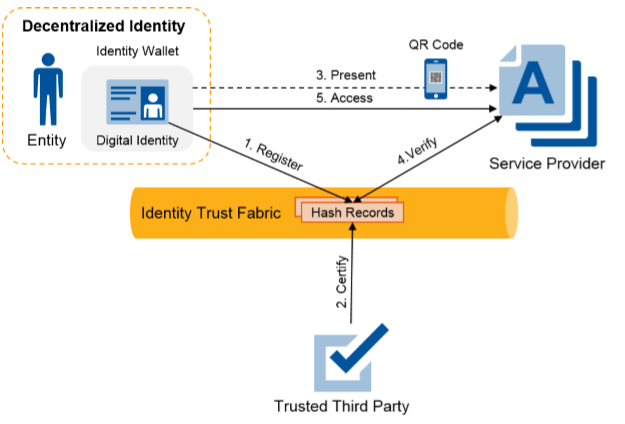
\includegraphics[width=0.9\columnwidth]{diag-comp-flussi.png} 
    \caption{Diagramma flussi tra i vari componenti}
    \label{fig:diag-flussi} 
\end{figure}
Si evidenziano essenzialmente due principali opzioni per la costruzione di questo applicativo. Il primo è l’utilizzo, anche per esso come per l’ITF, di un approccio totalmente distribuito basato su blockchain.  Il secondo approccio consiste i un’applicazione tradizionale.  
\subsubsection{Sviluppo distribuito}  
Questo approccio prevede che la logica applicativa sia totalmente affidata a codice eseguito su blockchain. Questo comporterebbe una disponibilità continuativa sempre garantita e altre caratteristiche di affidabilità e sicurezza. Come punto negativo si evidenzia che una soluzione del genere implicherebbe l’uso di molte tecnologie non completamente mature e di linguaggi in molti casi incompleti. Inoltre questa scelta implicherebbe l’utilizzo della stessa blockchain presente nell’ITF. I vantaggi attribuibili a questo approccio non sono considerati fondamentali al fine di una buona implementazione del SP, di contro gli svantaggi risultano particolarmente pesanti. L’applicazione di un approccio di questo genere anche se possibile risulta sconsigliato. Uno sviluppo di questo tipo, almeno in reti di tipo Permissionless, comporta un cambio di stile di programmazione dovuto all’alto costo delle operazioni. Come descritto nello studio tecnologico Ethereum ciò comporta le seguenti diversità:
\begin{itemize}
    \item alcuni pattern non risultano applicabili;
    \item complessità lineari sono difficilmente giustificabili;
    \item uso di pattern ad hoc.
\end{itemize}
\subsubsection{Sviluppo tradizionale}
La seconda opzione risulta essere una più tradizionale applicazione server che comunica tramite librerie alla blockchain. Si consiglia l’uso di linguaggi fortemente tipati quali: 
\begin{itemize}
    \item C++;
    \item C Sharp;
    \item Java.
\end{itemize}
Data l’alta diffusione di Javascript e NodeJS nella comunità Ethereum si consigliano pure questi.
In base al linguaggio scelto e alla tecnologia blockchain scelta, si dovranno utilizzare differenti librerie per effettuare la comunicazione tra la rete e l’applicativo. Nel caso di Ethereum si propongono le seguenti librerie:
\begin{table}[!h] %
    \caption{Tabella comparivi linguaggio per sviluppo SP}
    \label{tab:comp-ling}
    \begin{tabularx}{\textwidth}{|l|l|l|X|}
    \hline
    \textbf{Linguaggio} & \textbf{Libreria} & \textbf{Note}\\
    \hline
    C++   & cpp-ethereum & - \\
    \hline
    C Sharp   & Nethereum & Questa soluzione si collega particolarmente bene alla scelta di Xamarin per l’IW. \\
    \hline
    JS e NodeJS   & Web3 & -\\
    \hline
    Java  & Web3j & -\\
    \hline
    \end{tabularx}
\end{table}%

Di seguito si procederà alla trattazione di alcuni degli strumenti che si ritengono più utili.
\paragraph{Nethereum}:è un tool che permette una facile integrazione con il client in applicazioni .NET. Fornisce una suite di librerie open source che aiutano a prototipare applicazione .NET velocemente. E’ disponibile anche nel sotto insieme Xamarin.  La documentazione è presente è sembra ben strutturata e di ottima qualità. Inoltre potrebbe rappresentare una buona soluzione in caso di scelta di Microsoft Azure Blockchain. Il sito del progetto è il seguente www.nethereum.com.   
\paragraph{Web3}: è una collezione di librerie che permettono di interagire con un nodo remoto o locale usando una connessione HTTP o IPC. Web3 è presente in npm, meteor, pure js. Per il suo funzionamento è necessario avere un client attivo nel proprio computer. Web3 supporta Mist e Metamask. Il sito del progetto è il seguente: web3js.readthedocs.io.
\paragraph{Web3J}: si tratta di una libreria analoga a Web3 per Java.
\paragraph{Mist}: è un browser sviluppato direttamente dal team Ethereum in grado di operare transazioni direttamente nella blockchain senza la necessità di possedere un intero nodo. È estremamente immaturo e non utilizzabile in produzione. Si riporta di seguito il sito del progetto: github.com/ethereum/mist.
\paragraph{Metamask}: è uno plugin disponibile per i browser Chrome, Firefox e Opera che permette di interfacciarsi alla rete Ethereum senza la necessità di eseguire in intero nodo della rete. Il plugin include un wallet con cui l’utente può inserire il proprio account tramite la chiave privata. Una volta inserito l’account il plugin farà da tramite tra l’applicazione e la rete.
In caso, invece, si opti per la scelta di Hyperledger la scelta risulterebbe molto più semplice in quanto la blockchain in questione fornisce un’API per la comunicazione REST.


\subsubsection{Scelta del client Ethereum}
Il client è un componente che implementa il protocollo di comunicazione di Ethereum. Ethereum diversamente da Hyperledger presenta una realtà molto varia e frastagliata. Solo dal punto di vista del client ci sono multiple implementazioni per differenti sistemi operativi ed in differenti linguaggi. Questa diversità viene vista dalla community come un indicatore di salute per l’intero ecosistema. Il protocollo in ogni caso è sempre lo stesso ed è definito nel così detto Yellow Paper in nota 5, in sostanza si basa sull’utilizzo di file Json. 
Fino al settembre 2016 erano presenti le alternative esposte in tabella \ref{tab:comp-client}.
\begin{table}[!h] %
    \caption{Tabella comparivi client Ethereum}
    \label{tab:comp-client}
    \begin{tabularx}{\textwidth}{|X|X|X|}
    \hline
    \textbf{Client} & \textbf{Linguaggio} & \textbf{Sviluppatore}\\
    \hline
    Go-ethereum   & Go & Ethereum Foundation \\
    \hline
    Parity   & Rust & Ethcore \\
    \hline
    Cpp-ethereum   & C++ & Ethereum Foundation\\
    \hline
    Pyethapp  & Python & Ethereum Foundation\\
    \hline
    Ethereumjs-lib  & Javascript & Ethereum Foundation\\
    \hline
    Ethereum(J)  & Java & <ether.camp>\\
    \hline
    Ruby-ethereum  & Ruby & Jan Xie\\
    \hline
    EthereumH  & Haskell & BlockApps\\
    \hline
    \end{tabularx}
\end{table}%
I client appena citati sono accessibili tramite apposite librerie, un buon esempio potrebbe essere web3 per Javascript.
\subsubsection{Scelta del client Hyperledger}
In caso si dovesse optare per una scelta basata su Hyperledger quale base dell’ITF bisognerà ricadere sull’unica soluzione proposta dal team di sviluppo, cioè quella di utilizzare direttamente una comunicazione REST. Il team offre uno strumento detto Composer con il quale si potrà definire un’interfaccia per operare la comunicazione REST. Al fine di poter gestire efficientemente queste chiamate lato applicazione SP si consigliano le librerie esposte in tabella \ref{tab:comp-client-hyp}.
\begin{table}[!h] %
    \caption{Tabella comparivi client Ethereum}
    \label{tab:comp-client-hyp}
    \begin{tabularx}{\textwidth}{|X|X|X|}
    \hline
    \textbf{Linguaggio} & \textbf{Librerie} & \textbf{Sito}\\
    \hline
    .NET   & WCF REST Starter Kit  & \url{www.asp.net/downloads/starter-kits/wcf-rest} \\
    \hline
    .NET   & OpenRasta & \url{www.openrasta.org} \\
    \hline
    .NET   & Service Stack  & \url{www.servicestack.net} \\
    \hline
    Java  & Jersey & \url{www.jersey.java.net} \\
    \hline
    Java  & RESREasy & \url{www.jboss.org/resteasy}\\
    \hline
    Java  & Restlet & \url{www.restlet.org}\\
    \hline
    C++  & linavajo & \url{www.libnavajo.org}\\
    \hline
    C++  & C++ RESTful framework & \url{www.github.com/corvusoft/restbed}\\
    \hline
    C++  & C++ REST SDK & \url{www.github.com/Microsoft/cpprestsdk}\\
    \hline
    \end{tabularx}
\end{table}%
Data l’amplissima diffusione delle API REST e di queste librerie non si procede ad una trattazione analitica.
\subsection{Conclusioni scelta sviluppo}
Considerando quanto precedentemente detto lo sviluppo tradizionale sembrerebbe avrebbe meno incognite e un ampio repertorio di librerie utilizzabili. Si propone, quindi un’architettura del secondo tipo.
Inoltre, si vuole fare notare come l’utilizzo delle soluzioni .NET potrebbero rivelarsi molto vantaggiose in quanto facilmente integrabili con il componente IW e Azure Blockchain.
\subsection{Motivazioni}
\subsubsection{Aspetti positivi}
A seguito dell’analisi sopra proposta sono stati individuati i seguenti aspetti positivi:
\begin{itemize}
    \item lo sviluppo di un’applicazione server tradizionale comporta uno sviluppo molto semplice e immediato, grazie anche alla disponibilità di un ampio repertorio di librerie;
    \item la comunicazione con la blockchain risulta in ogni caso facilmente implementabile grazie all’utilizzo di apposite librerie.
    \item esiste un’ampia scelta di librerie front end per ogni possibile linguaggio di sviluppo.
\end{itemize}
    
\subsubsection{Fattori di rischio}
\begin{risk}{Inesperienza nello sviluppo C Sharp}
    \riskdescription{Non si ha esperienza nello sviluppo di applicazioni C Sharp.}
    \risksolution{Rendere edotto il responsabili del progetto, il quale mettera a disposizione del personale per impartire supporto su C Sharp.}
    \label{risk:centralization-vision-from-user} 
\end{risk}
\begin{risk}{difficoltà di integrazione con Monokee}
    \riskdescription{Il componete SP è il componente che deve essere integrato in Monokee}
    \risksolution{Rendere edotto il responsabili del progetto, il quale metterà a disposizione del personale.}
    \label{risk:centralization-vision-from-user} 
\end{risk}
\begin{risk}{Prestazioni chiamate alla rete blockchain}
    \riskdescription{Il componete SP deve interrogare la rete blockchain, questo potrebbe rappresentare un problema di performance}
    \risksolution{Rendere edotto il responsabili del progetto, valutare soluzioni alternative.}
    \label{risk:centralization-vision-from-user} 
\end{risk}
\subsection{Conclusioni}
Dal presente studio emerge come la creazione di un SP sviluppato come applicativo server, e non come applicazione distribuita, possa essere un’ottima opzione implementativa. Lo studio non presenta particolari rischi. In definitiva, si ritiene che un approccio di questo tipo sia fattibile nei tempi dello stage.
%**************************************************************

\section{Obiettivi}

Scopo delle attività di stage è il raggiungimento dei seguenti obiettivi.\\
\paragraph{Obiettivi minimi}
\begin{itemize}
    \item codifica dei moduli SP e IW;
    \item documenti di analisi dei requisiti;
    \item documenti di architettura.
\end{itemize}
    
\paragraph{Obiettivi opzionali}
\begin{itemize}
    \item documenti di progettazione;
    \item documenti di testing;
    \item documenti di validazione (anomalie e bug).
\end{itemize}
    

%**************************************************************
\section{Pianificazione}
Il lavoro durante lo stage è stato svolto seguendo la seguente pianificazione iniziale:
\begin{itemize}
    

\item \textbf{Studio Fattibilità} (40 ore): questa fase è focalizzata allo studio della tecnologia Blockchain da adottare e il suo impiego nello specifico caso d’uso.  La valutazione verrà effettuata valutando le capacità di utilizzo delle tecnologie e interpretazione delle informazioni.

    Prodotti attesi: 
    \begin{enumerate}
        \item Documento: Monokee – Identity Wallet, studio di Fattibilità
        \item Documento: Monokee – Service Provider, studio di fattibilità
    \end{enumerate}
        

\item \textbf{Analisi requisiti} (40 ore): al termine di questo periodo i casi d'uso saranno definiti e si avrà il tracciamento requisiti-casi d'uso.
    I requisiti saranno una rappresentazione delle 5 funzionalità core che i moduli dovranno erogare:
    \begin{enumerate}
        \item Registrazione: il wallet crea l’identità digitale dell’utente e ne associa una chiave privata e pubblica; interagisce quindi con il componente ITF per registrare l’associazione Identità-Service Provider . 
        \item Certificazione (da capire il coinvolgimento del Wallet e del Service Provider): un ente terzo può validare l’identità dell’utente tramite un processo di “identity proofing);  in caso di validazione positiva l’ente terzo può certificare l’identità (o una parte degli attributi del profilo) firmandoli con la propria chiave privata
        \item Presentazione: la chiave pubblica e il riferimento a dove trovarne l’hash viene inviato al Service Provider; il fornitore del servizio a questo punto può chiedere l’invio di ulteriori attributi dell’utente che possono essere presenti nel suo wallet; gli attributi verranno inviati firmati tramite QR-Code
        \item Verifica: il Service Provider utilizza le informazioni ricevute per verificare l’identità e gli attributi tramite un confronto dei valori hash nell’ITF.
        \item Access: a seguito di una verifica positiva dell’identità il provider dei servizi concede l’accesso all’applicazione/servizio.
    \end{enumerate}
    
    


 
    Prodotti attesi: 
    \begin{enumerate}
        \item Documento: Monokee – Identity Wallet,  analisi e specifica dei requisiti
        \item Documento: Monokee – Service Provider,  analisi e specifica dei requisiti
    \end{enumerate}
    

\item \textbf{Progettazione architetturale} (40 ore): avrà come risultato l'architettura generale che implementa le funzionalità rilevate dai casi d'uso. La valutazione verrà effettuata valutando le capacità di progettazione di un'architettura a partire dalle funzionalità individuate;
Prodotti attesi: 
    \begin{enumerate}
        \item Documento: Monokee – Identity Wallet, architettura
        \item Documento: Monokee – Service provider, architettura
    \end{enumerate}
    

\item \textbf{Progettazione dettaglio} (60 ore): come risultato si avrà la definizione dei metodi in pseudo-codice. La valutazione verrà effettuata valutando le capacità di traduzione in pseudo-codice dell'architettura progettata
        Prodotti attesi:
        \begin{enumerate}
            \item Documento: Monokee – Identity Wallet, progettazione
            \item Documento: Monokee – Service Provider, progettazione
        \end{enumerate}
            

\item \textbf{Codifica e Verifica} (120 ore): sarà realizzata la codifica dei metodi e saranno effettuati i test di unità e integrazione. La valutazione verrà effettuata valutando l'apprendimento e la capacità di implementazione della tecnologia scelta;
Prodotti attesi: 
        \begin{enumerate}
            \item Sorgenti del modulo Identity Wallet basati su tecnologia mobile (da valutare l’implementazione tramite Xamarin o strumenti nativi)
            \item Sorgenti del modulo Service Provider
            \item Documento: Monokee – Identity Wallet, testing
            \item Documento: Monokee – Service Provider, testing
        \end{enumerate}
    

\item \textbf{Validazione} (20 ore): al termine si avrà il prodotto software richiesto. Verrà valutato il software risultante tramite fase di testing.
    Prodotti attesi: 
    \begin{enumerate}
        \item Documento: Monokee – Identity Wallet, anomalie e bug
        \item Documento: Monokee – Service Provider, anomalie e bug 
    \end{enumerate}
    
\end{itemize}